\begin{frame}\begin{center}
\LARGE\textbf{Randomization}
\end{center}\end{frame}
%-------------------------------------------------------------------------------
%-------------------------------------------------------------------------------
\begin{frame}\textbf{Treatment Status}\vspace{0.3cm}

\begin{align*}
D &\qquad \text{self-selected} \\
\xi &\qquad \text{assigned} \\
A &\qquad  \text{actual}
\end{align*}
\end{frame}
%-------------------------------------------------------------------------------
%-------------------------------------------------------------------------------
\begin{frame}\textbf{Key Identifying Assumptions}\vspace{0.3cm}
\begin{align*}
(Y_1, Y_0) & \indep D \\
(Y_1, Y_0) & \indep \xi \\
(Y_1, Y_0) & \indep A
\end{align*}

When do we have to worry about compliance?

\end{frame}
%-------------------------------------------------------------------------------
%-------------------------------------------------------------------------------
\begin{frame}
\begin{align*}
& E(Y\mid A = 1) - E(Y\mid A = 0) \\
& \qquad = E(Y_1\mid A = 1) - E(Y_0\mid A = 0)  \tag{by full compliance} \\
& \qquad = E(Y_1) - E(Y_0)  \tag{by randomization} \\
& \qquad = B^{ATE} = B^{TT} = B^{TUT}
\end{align*}
\end{frame}
%-------------------------------------------------------------------------------
%-------------------------------------------------------------------------------
\begin{frame}
\begin{figure}\caption{Distribution of Effects}
\scalebox{0.35}{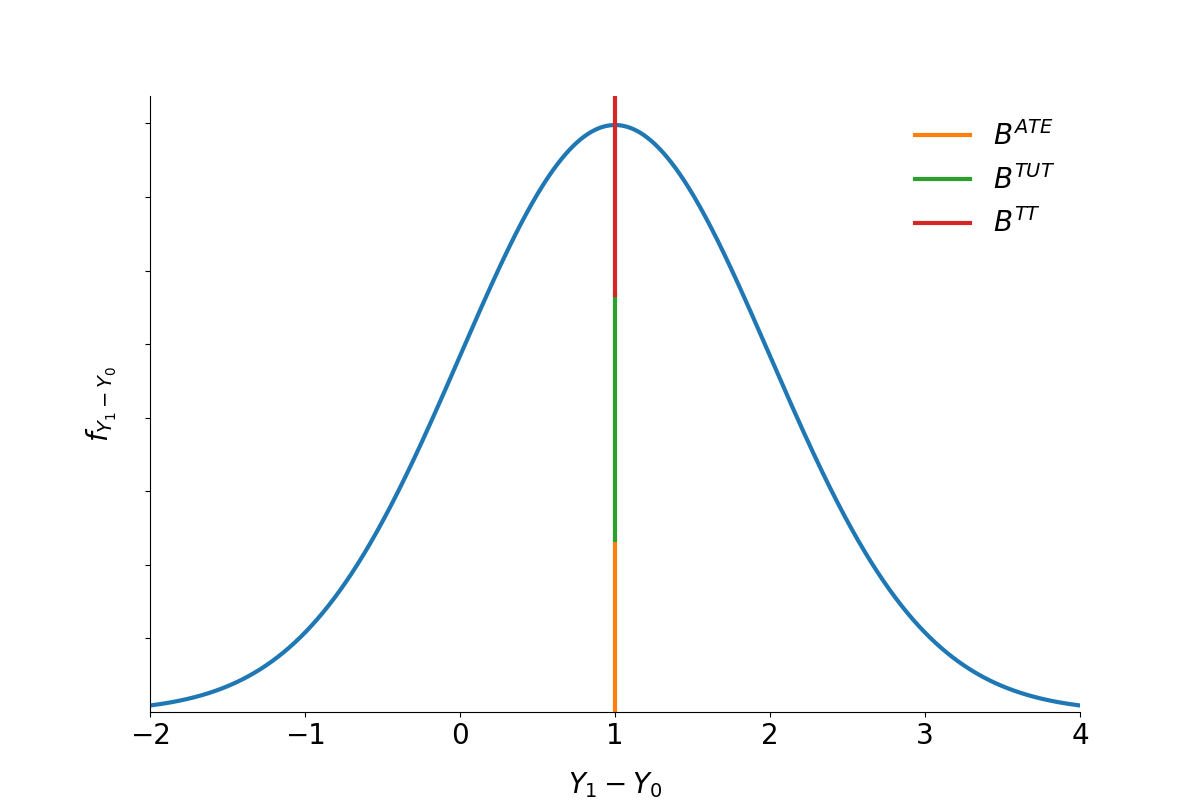
\includegraphics{fig-treatment-effects-without-eh}}
\end{figure}
\end{frame}
%-------------------------------------------------------------------------------
%-------------------------------------------------------------------------------
\begin{frame}
What if we can only deny program participation to individuals who are willing to participate?
\begin{align*}
& E(Y\mid D= 1, A = 1) - E(Y\mid D = 1, A = 0) \\
& \qquad\qquad = E(Y_1\mid D= 1, A = 1) - E(Y_0\mid D=1, A = 0) \\
& \qquad\qquad = E(Y_1\mid D = 1) - E(Y_0 \mid D = 1)  \\
& \qquad\qquad = B^{TT} \neq B^{ATE} \neq B^{TUT}
\end{align*}
\end{frame}
%-------------------------------------------------------------------------------
%-------------------------------------------------------------------------------
\begin{frame}\textbf{Issues}\vspace{0.3cm}

\begin{itemize}\setlength\itemsep{1em}
\item compliance
\item imperfect randomization
\item ethical concerns
\item feasibility
\item expenses
\item external validity
\end{itemize}
\end{frame}
%-------------------------------------------------------------------------------
%-------------------------------------------------------------------------------
\begin{frame}\textbf{Challenges to Scaling Experiments}\vspace{0.3cm}

\begin{itemize}\setlength\itemsep{1em}
\item market equilibrium effects
\item spillovers
\item political reactions
\item context dependence
\item randomization or site-selection bias
\item piloting bias\vspace{0.3cm}
\end{itemize}

See \citeA{Banerjee.2017} for a discussion of these challenges and their attempts to address them in their work.
\end{frame}

%-------------------------------------------------------------------------------
%-------------------------------------------------------------------------------
